%-----------------------------------------------------------------------
% Simulating incompressible flow over terrain - user guide
%-----------------------------------------------------------------------
\documentclass[11pt]{article}
% \usepackage[bookmarks=true]{hyperref}  % this changes the page location !
\usepackage[bookmarks=true,colorlinks=true,linkcolor=blue]{hyperref}

% \input documentationPageSize.tex
\hbadness=10000 
\sloppy \hfuzz=30pt

% \voffset=-.25truein
% \hoffset=-1.25truein
% \setlength{\textwidth}{7in}      % page width
% \setlength{\textheight}{9.5in}    % page height

\usepackage{calc}
\usepackage[lmargin=.75in,rmargin=.75in,tmargin=.75in,bmargin=.75in]{geometry}

\input homeHenshaw

% \input{pstricks}\input{pst-node}
% \input{colours}
\newcommand{\blue}{\color{blue}}
\newcommand{\green}{\color{green}}
\newcommand{\red}{\color{red}}
\newcommand{\black}{\color{black}}


\usepackage{amsmath}
\usepackage{amssymb}

\usepackage{verbatim}
\usepackage{moreverb}

\usepackage{graphics}    
\usepackage{epsfig}    
\usepackage{calc}
\usepackage{ifthen}
\usepackage{float}
% the next one cause the table of contents to disappear!
% * \usepackage{fancybox}

\usepackage{makeidx} % index
\makeindex
\newcommand{\Index}[1]{#1\index{#1}}

\usepackage{tikz}
% \usepackage{pgfplots}
\input trimFig.tex


% ---- we have lemmas and theorems in this paper ----
\newtheorem{assumption}{Assumption}
\newtheorem{definition}{Definition}

% \newcommand{\homeHenshaw}{/home/henshaw.0}

\newcommand{\Overture}{{\bf Over\-ture\ }}
\newcommand{\ogenDir}{\homeHenshaw/Overture/ogen}

\newcommand{\cgDoc}{\homeHenshaw/cgDoc}
\newcommand{\vpDir}{\homeHenshaw/cgDoc/ins/viscoPlastic}

\newcommand{\ovFigures}{\homeHenshaw/OvertureFigures}
\newcommand{\obFigures}{\homeHenshaw/res/OverBlown/docFigures}  % for figures
\newcommand{\convDir}{\homeHenshaw/cgDoc/ins/tables}
\newcommand{\insDocDir}{\homeHenshaw/cgDoc/ins}

% *** See http://www.eng.cam.ac.uk/help/tpl/textprocessing/squeeze.html
% By default, LaTeX doesn't like to fill more than 0.7 of a text page with tables and graphics, nor does it like too many figures per page. This behaviour can be changed by placing lines like the following before \begin{document}

\renewcommand\floatpagefraction{.99}
\renewcommand\topfraction{.99}
\renewcommand\bottomfraction{.99}
\renewcommand\textfraction{.01}   
\setcounter{totalnumber}{50}
\setcounter{topnumber}{50}
\setcounter{bottomnumber}{50}

\begin{document}

\input wdhDefinitions.tex

\def\comma  {~~~,~~}
\newcommand{\uvd}{\mathbf{U}}
\def\ud     {{    U}}
\def\pd     {{    P}}
\def\calo{{\cal O}}

\newcommand{\mbar}{\bar{m}}
\newcommand{\Rbar}{\bar{R}}
\newcommand{\Ru}{R_u}         % universal gas constant
% \newcommand{\Iv}{{\bf I}}
% \newcommand{\qv}{{\bf q}}
\newcommand{\Div}{\grad\cdot}
\newcommand{\tauv}{\boldsymbol{\tau}}
\newcommand{\thetav}{\boldsymbol{\theta}}
% \newcommand{\omegav}{\mathbf{\omega}}
% \newcommand{\Omegav}{\mathbf{\Omega}}

\newcommand{\Omegav}{\boldsymbol{\Omega}}
\newcommand{\omegav}{\boldsymbol{\omega}}
\newcommand{\sigmav}{\boldsymbol{\sigma}}
\newcommand{\cm}{{\rm cm}}

\newcommand{\ds}{\Delta s}
\newcommand{\dsbl}{\ds_{\rm bl}}


\newcommand{\sumi}{\sum_{i=1}^n}
% \newcommand{\half}{{1\over2}}
\newcommand{\dt}{{\Delta t}}

\def\ff {\tt} % font for fortran variables

% define the clipFig commands:
%% \input clipFig.tex

\newcommand{\Bc}{{\mathcal B}}
\newcommand{\Dc}{{\mathcal D}}
\newcommand{\Ec}{{\mathcal E}}
\newcommand{\Fc}{{\mathcal F}}
\newcommand{\Gc}{{\mathcal G}}
\newcommand{\Hc}{{\mathcal H}}
\newcommand{\Ic}{{\mathcal I}}
\newcommand{\Jc}{{\mathcal J}}
\newcommand{\Lc}{{\mathcal L}}
\newcommand{\Nc}{{\mathcal N}}
\newcommand{\Pc}{{\mathcal P}}
\newcommand{\Rc}{{\mathcal R}}
\newcommand{\Sc}{{\mathcal S}}

\newcommand{\bogus}[1]{}  % removes is argument completely

\vspace{5\baselineskip}
\begin{flushleft}
{\LARGE
Simulating Airflow over Terrain using Overture's Cgins Solver\\
}
\vspace{2\baselineskip}
Kyle. K. Chand,    \\
William D. Henshaw, \\
Charles M. Reid, 
~\footnote{This work was performed under the auspices of the U.S. Department of Energy (DOE) by
Lawrence Livermore National Laboratory under Contract DE-AC52-07NA27344 and by 
DOE contracts from the ASCR Applied Math Program.}  \\
% Centre for Applied Scientific Computing  \\
Lawrence Livermore National Laboratory      \\
Livermore, CA, 94551.  \\
\vspace{\baselineskip}
\today\\
\vspace{\baselineskip}
LLNL-?????

\vspace{4\baselineskip}

\noindent{\bf\large Abstract:}

This document describes how to (1) obtain terrain data (elevation data) from the USGS National Map Viewer for a specified region,
(2) generate an overlapping grid for this region using Ogen, and (3) simulate the air flow over the terrain
using the Cgins incompressible flow solver.

\end{flushleft}

% \clearpage
\tableofcontents
% \listoffigures

\vfill\eject


\section{Introduction}

Cgins is an incompressible flow solver built upon the Overture framework.
Cgins solves the incompressible Navier-Stokes equations (with Boussinesq approimation
for temperature dependent buoyant flows). See~\cite{CginsUserGuide} and~\cite{CginsReferenceManual} for further 
details. 

The steps for simulating flow over some specified terrain are as follows. 
\begin{enumerate}
  \item Obtain terrain (elevation) data for the domain of interest 
     from the National Elevation Dataset (NED) available from the USGS {\em National Map Viewer} web site.
  \item Use the {\tt readTerrain.m} matlab script to convert the USGS terrain data (in longitude-latitude coordinates)
       into horizontal coordinates measured in meters and output the result in a data file with format understood by
       the Overture NURBS mapping. 
  \item Use the Ogen script {\tt terrainGrid.cmd} to generate an overlapping grid, using the terrain data file from step 2.
  \item Use the Cgins script {\tt terrain.cmd} to simulate the flow using Cgins.
\end{enumerate}
These steps are described in further detail 
in the following sections. Note the relevant scripts ({\tt readTerrain.m}, {\tt terrainGrid.cmd}
and {\tt terrain.cmd}) can be found in 
the directory {\tt cg/ins/runs/terrain} of the CG distribution. 



%- Q: How do I locate and download National Elevation Dataset (NED) products using The National Map Viewer?
%- 
%- A: Bare earth digital elevation model (DEM) data from the NED, previously available through the Seamless Server Viewer, is accessed in The National Map Viewer with the 'Download Data' tool. Use the following procedures to download DEM data:
%- 
%-  1.   Zoom to your area of interest.
%-  2.   Click the Download Data tool near the top right corner of the viewer banner.
%-  3.   Use the current map extent, choose a reference area polygon from the Download options dropdown menu, or create your own custom polygon.
%-     Select the data theme of Elevation and product format.
%-     Select available NED products, such as 2 arc-second (Alaska only), 1 arc-second (conterminous U.S., Hawaii, Puerto Rico, portions of Alaska, western & southern Canada along U.S. border, and all of Mexico), 1/3 arc-second (conterminous U.S., Hawaii, and portions of Alaska), or 1/9 arc-second (in limited areas of U.S. only).
%-     Add selected products to the Cart.
%-     Checkout and enter your e-mail address twice to place your order. 

% ================================================================================================================
\section{Obtaining terrain (elevation) data from the USGS National Map Viewer} \label{sec:NationalMapViewer}


 Terrain data for a specified region can be obtain from the USGS
{\em National Map Viewer}. Here are the steps.

\begin{enumerate}
  \item Goto to {\tt http://viewer.nationalmap.gov/viewer/}. (For help see {\tt http://\-nationalmap.gov/\-viewer.html}).
  \item Zoom on the map to locate your area of interest (see Figure~\ref{fig:NationalMapViewer}(a)). The pointer coordinates
(shown near the bottom) indicate the latitude/longitude of the pointer's current
location. This can be used to locate map coordinates for particular
latitudes and longitudes. Normally for Cgins you would choose a region that is
say 1-10 kilometers on a side.
  \item Choose the {\tt Download Data} button (near the top).
  \item Choose {\tt click here} to download the current map extent.
  \item Check the box to the left of the {\tt Elevation} theme and select {\tt GridFloat} in the options to the right (see Figure~\ref{fig:NationalMapViewer}(b)). 
  \item You may also want to check the box to the left of {\tt US Topo} to get a topographic figure (pdf file) of a region that 
    includes the domain you selected,
    or else save the image from the web-browser by printing to a file (this is how map on the right of Figure~\ref{fig:AltamontPass} was created).
  \item Enter {\tt next}.
  \item Select the box beside {\em National Elevation DataSet (NED) (1/3 arc second)} (see Figure~\ref{fig:NationalMapViewer}(c)).  
        You may also choose higher resolution {\em 1/9 Arc Second} or lower resolution, {\em 1 Arc Second}, if available. {\bf NOTE:} Choosing {\em Pre-packaged Float format} will NOT return the selected region
      but rather a larger region that contains the domain of interest. 
   \item Enter {\tt next}.
   \item On the left panel choose {\tt Checkout} (there is no cost).
   \item On the left panel enter your email address and choose {\tt Place Order} (see Figure~\ref{fig:NationalMapViewer}(d)).
   \item You will receive an email with a download link. Download the file and unzip it. This will create
       a subdirectory (e.g. NED\textunderscore81691785). 
   \item The {\tt readTerrain.m} matlab script (see section~\ref{sec:readTerrain}) 
         will read two files in this sub-directory, e.g. {\tt NED\textunderscore81691785/ned\textunderscore81691785.hdr} (short header text file) 
         and {\tt NED\textunderscore81691785/ned\textunderscore81691785.flt} (elevation data). 
\end{enumerate}

{\bf Notes:}
\begin{enumerate}
  \item With the `Index 24K'' option (at step 3. above) you can click on the map to choose an area outlined by  green lines.
\end{enumerate}

{%%%
\newcommand{\figWidthb}{9.cm}
\newcommand{\trimfigb}[2]{\trimPlot{#1}{#2}{.0}{.0}{.0}{.0}}
% 
% % -----------------------------------------------------------------------------------------------------------------------------------------
\begin{figure}[hbt]
\begin{center}
\begin{tikzpicture}[scale=1]
  \useasboundingbox (0,.5) rectangle (18.,12);  % set the bounding box (so we have less surrounding white space)
%
\draw ( 0.,6.0)  node[anchor=south west,xshift=-4pt,yshift=+0pt] {\trimfigb{fig/NationalMapFig1}{\figWidthb}};
\draw ( 0.,6.0) node[draw,fill=white,anchor=south west,xshift=+2pt,yshift=+4pt] {\scriptsize (a) select view};
%
\draw (9.2,6.0)  node[anchor=south west,xshift=-4pt,yshift=+0pt] {\trimfigb{fig/NationalMapFig2}{\figWidthb}};
\draw (9.2,6.0) node[draw,fill=white,anchor=south west,xshift=+2pt,yshift=+4pt] {\scriptsize (b) select data format};
%
\draw ( 0.,0.0)  node[anchor=south west,xshift=-4pt,yshift=+0pt] {\trimfigb{fig/NationalMapFig3}{\figWidthb}};
\draw ( 0.,0.0) node[draw,fill=white,anchor=south west,xshift=+2pt,yshift=+4pt] {\scriptsize (c) select arc second resolution};
%
\draw (9.2,0.0)  node[anchor=south west,xshift=-4pt,yshift=+0pt] {\trimfigb{fig/NationalMapFig4}{\figWidthb}};
\draw (9.2,0.0) node[draw,fill=white,anchor=south west,xshift=+2pt,yshift=+4pt] {\scriptsize (d) check-out (free)};
%
% \draw (current bounding box.south west) rectangle (current bounding box.north east);
%grid:
% \draw[step=1cm,gray] (0,0) grid (18,12.);
\end{tikzpicture}
\end{center}
 \caption{The National Map Viewer can be used to download terrain data.
   (a) viewport after zooming to select a region of interest.
   (b) selecting a format for the data set.
   (c) selecting the arc second resolution of the data set.
   (d) {\em check-out} (it's free of charge). 
     }
  \label{fig:NationalMapViewer}
\end{figure}
% -----------------------------------------------------------------------------------------------------------------------------------------------
%
}%

%- 
%- 
%- \newcommand{\mapFigWidth}{15cm}
%- \begin{figure}
%- \begin{centering}
%- 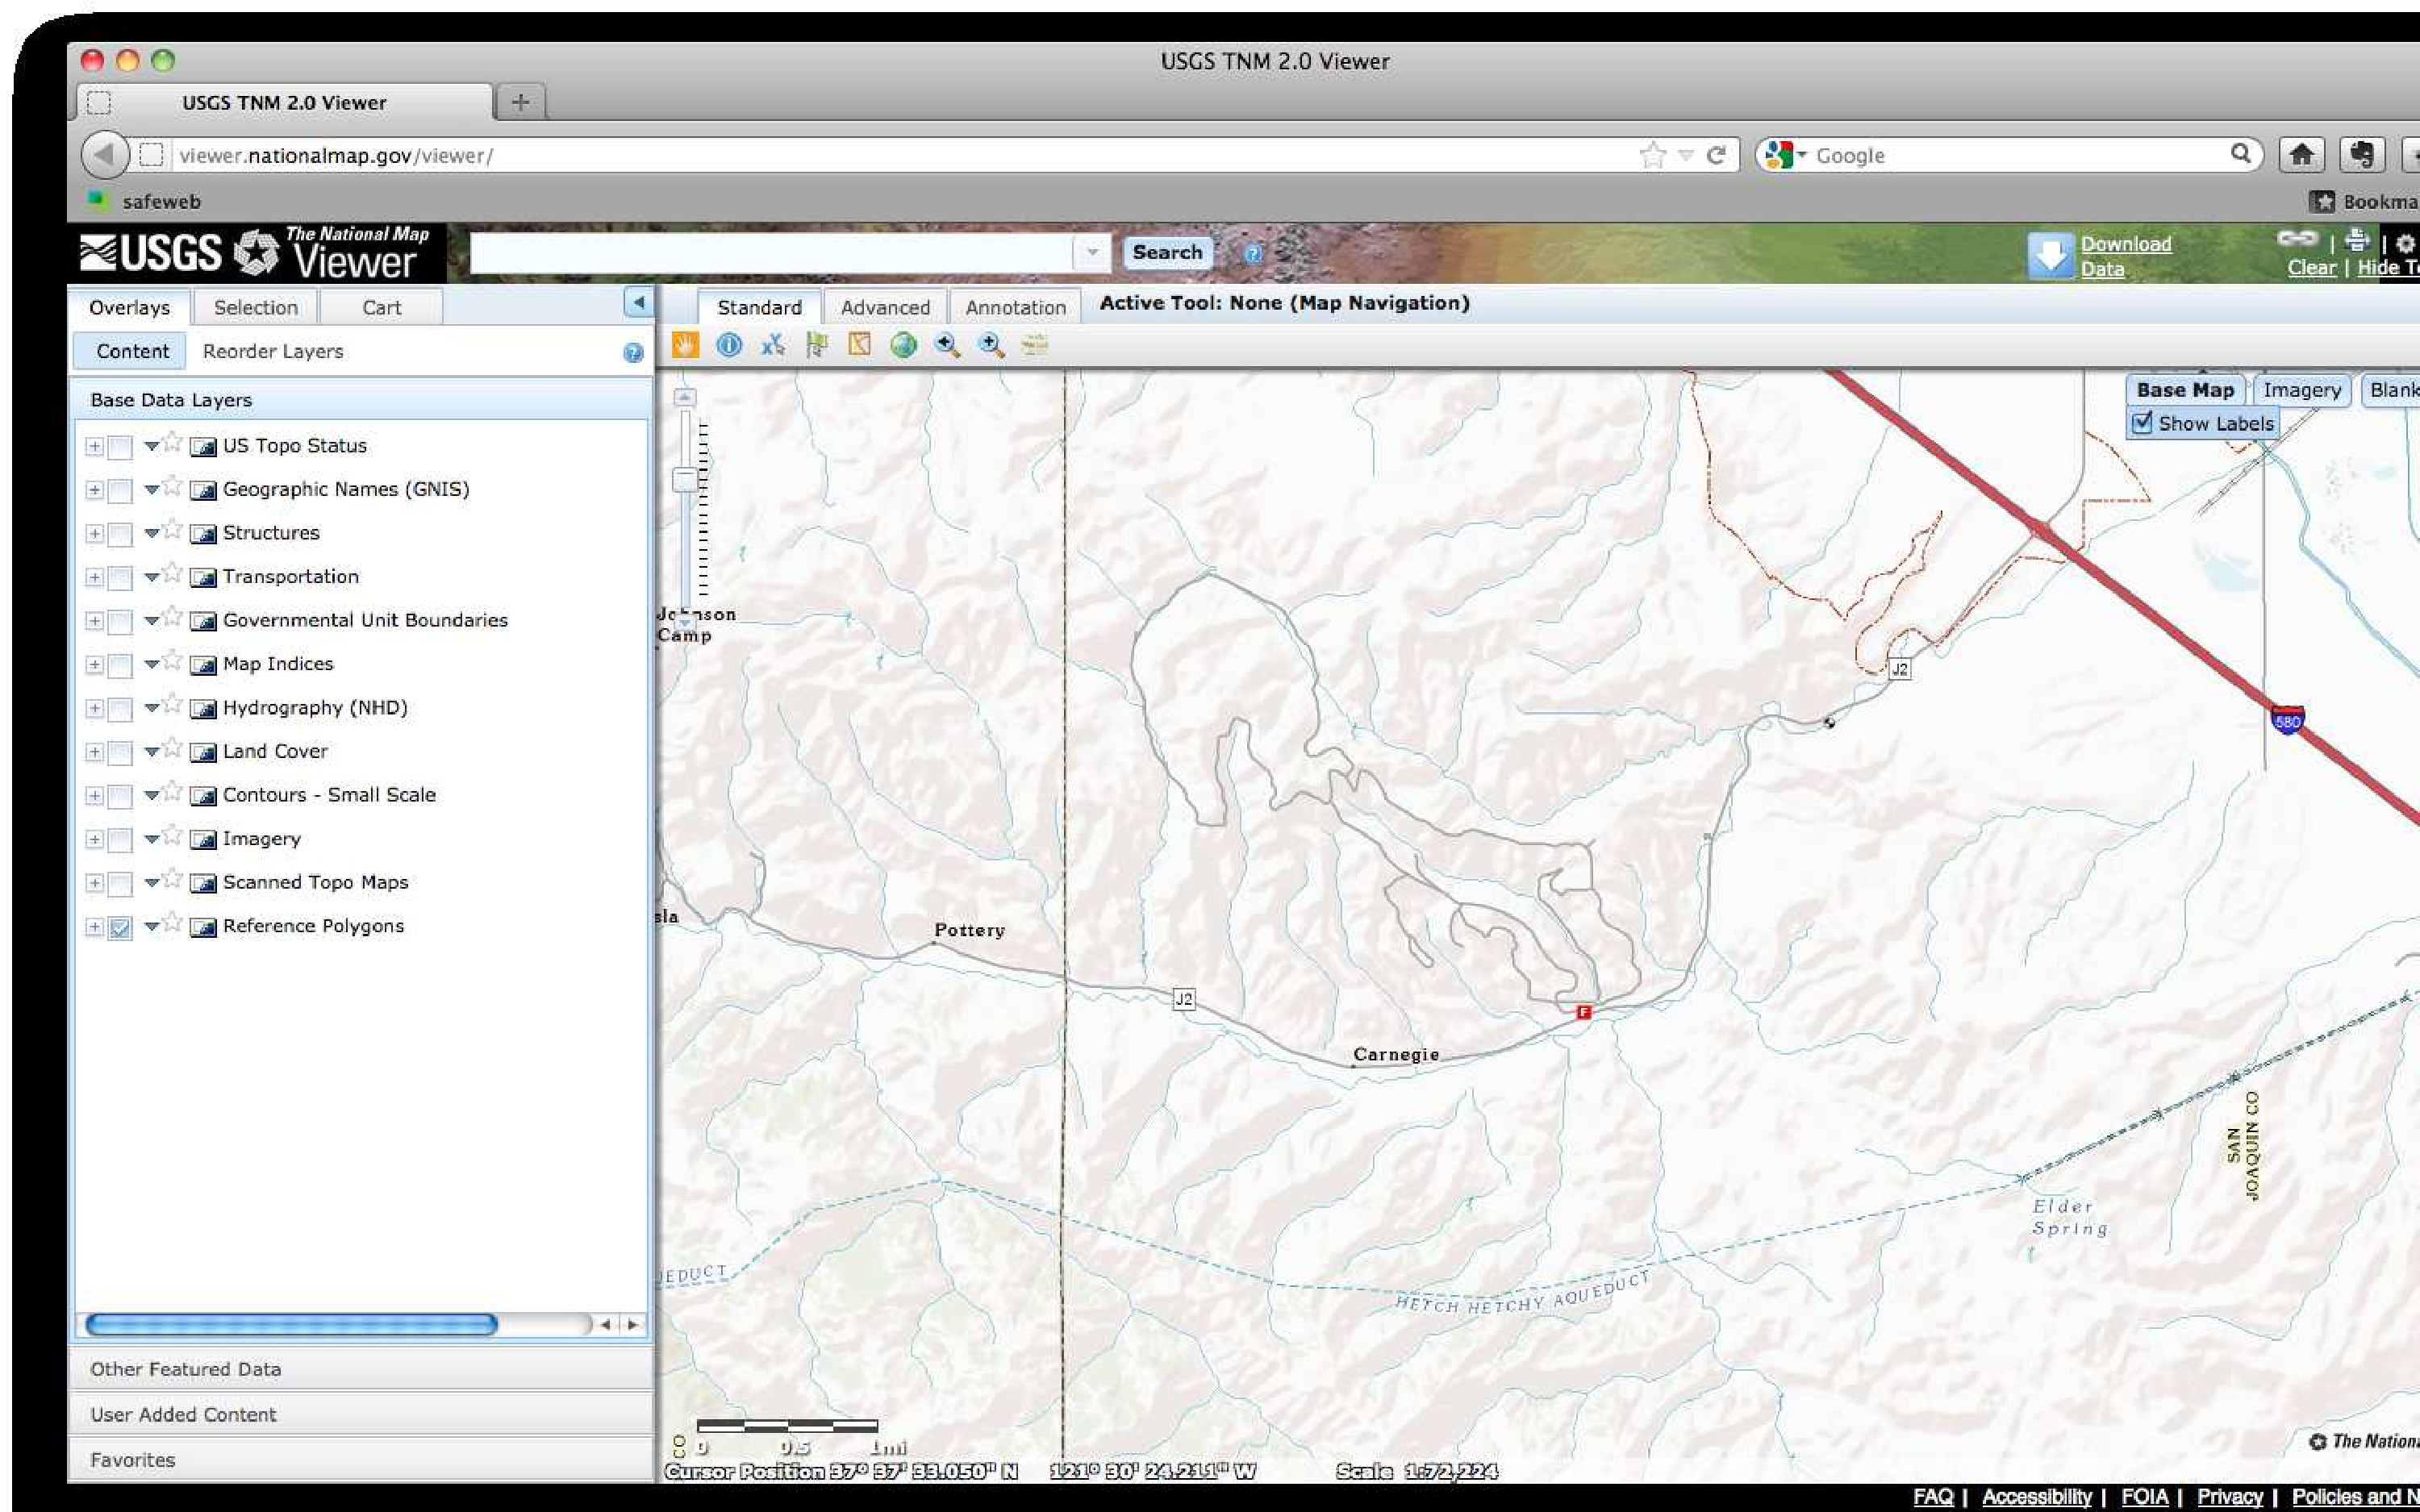
\includegraphics[width=\mapFigWidth]{fig/NationalMapFig1}
%- \par\end{centering}
%- 
%- \caption{\label{fig:Region-of-interest}The National Map Viewer can be used to download terrain data. This figure
%-     shows the viewport after zooming to select a region of interest.}
%- \end{figure}
%- 
%- \begin{figure}
%- \begin{centering}
%- 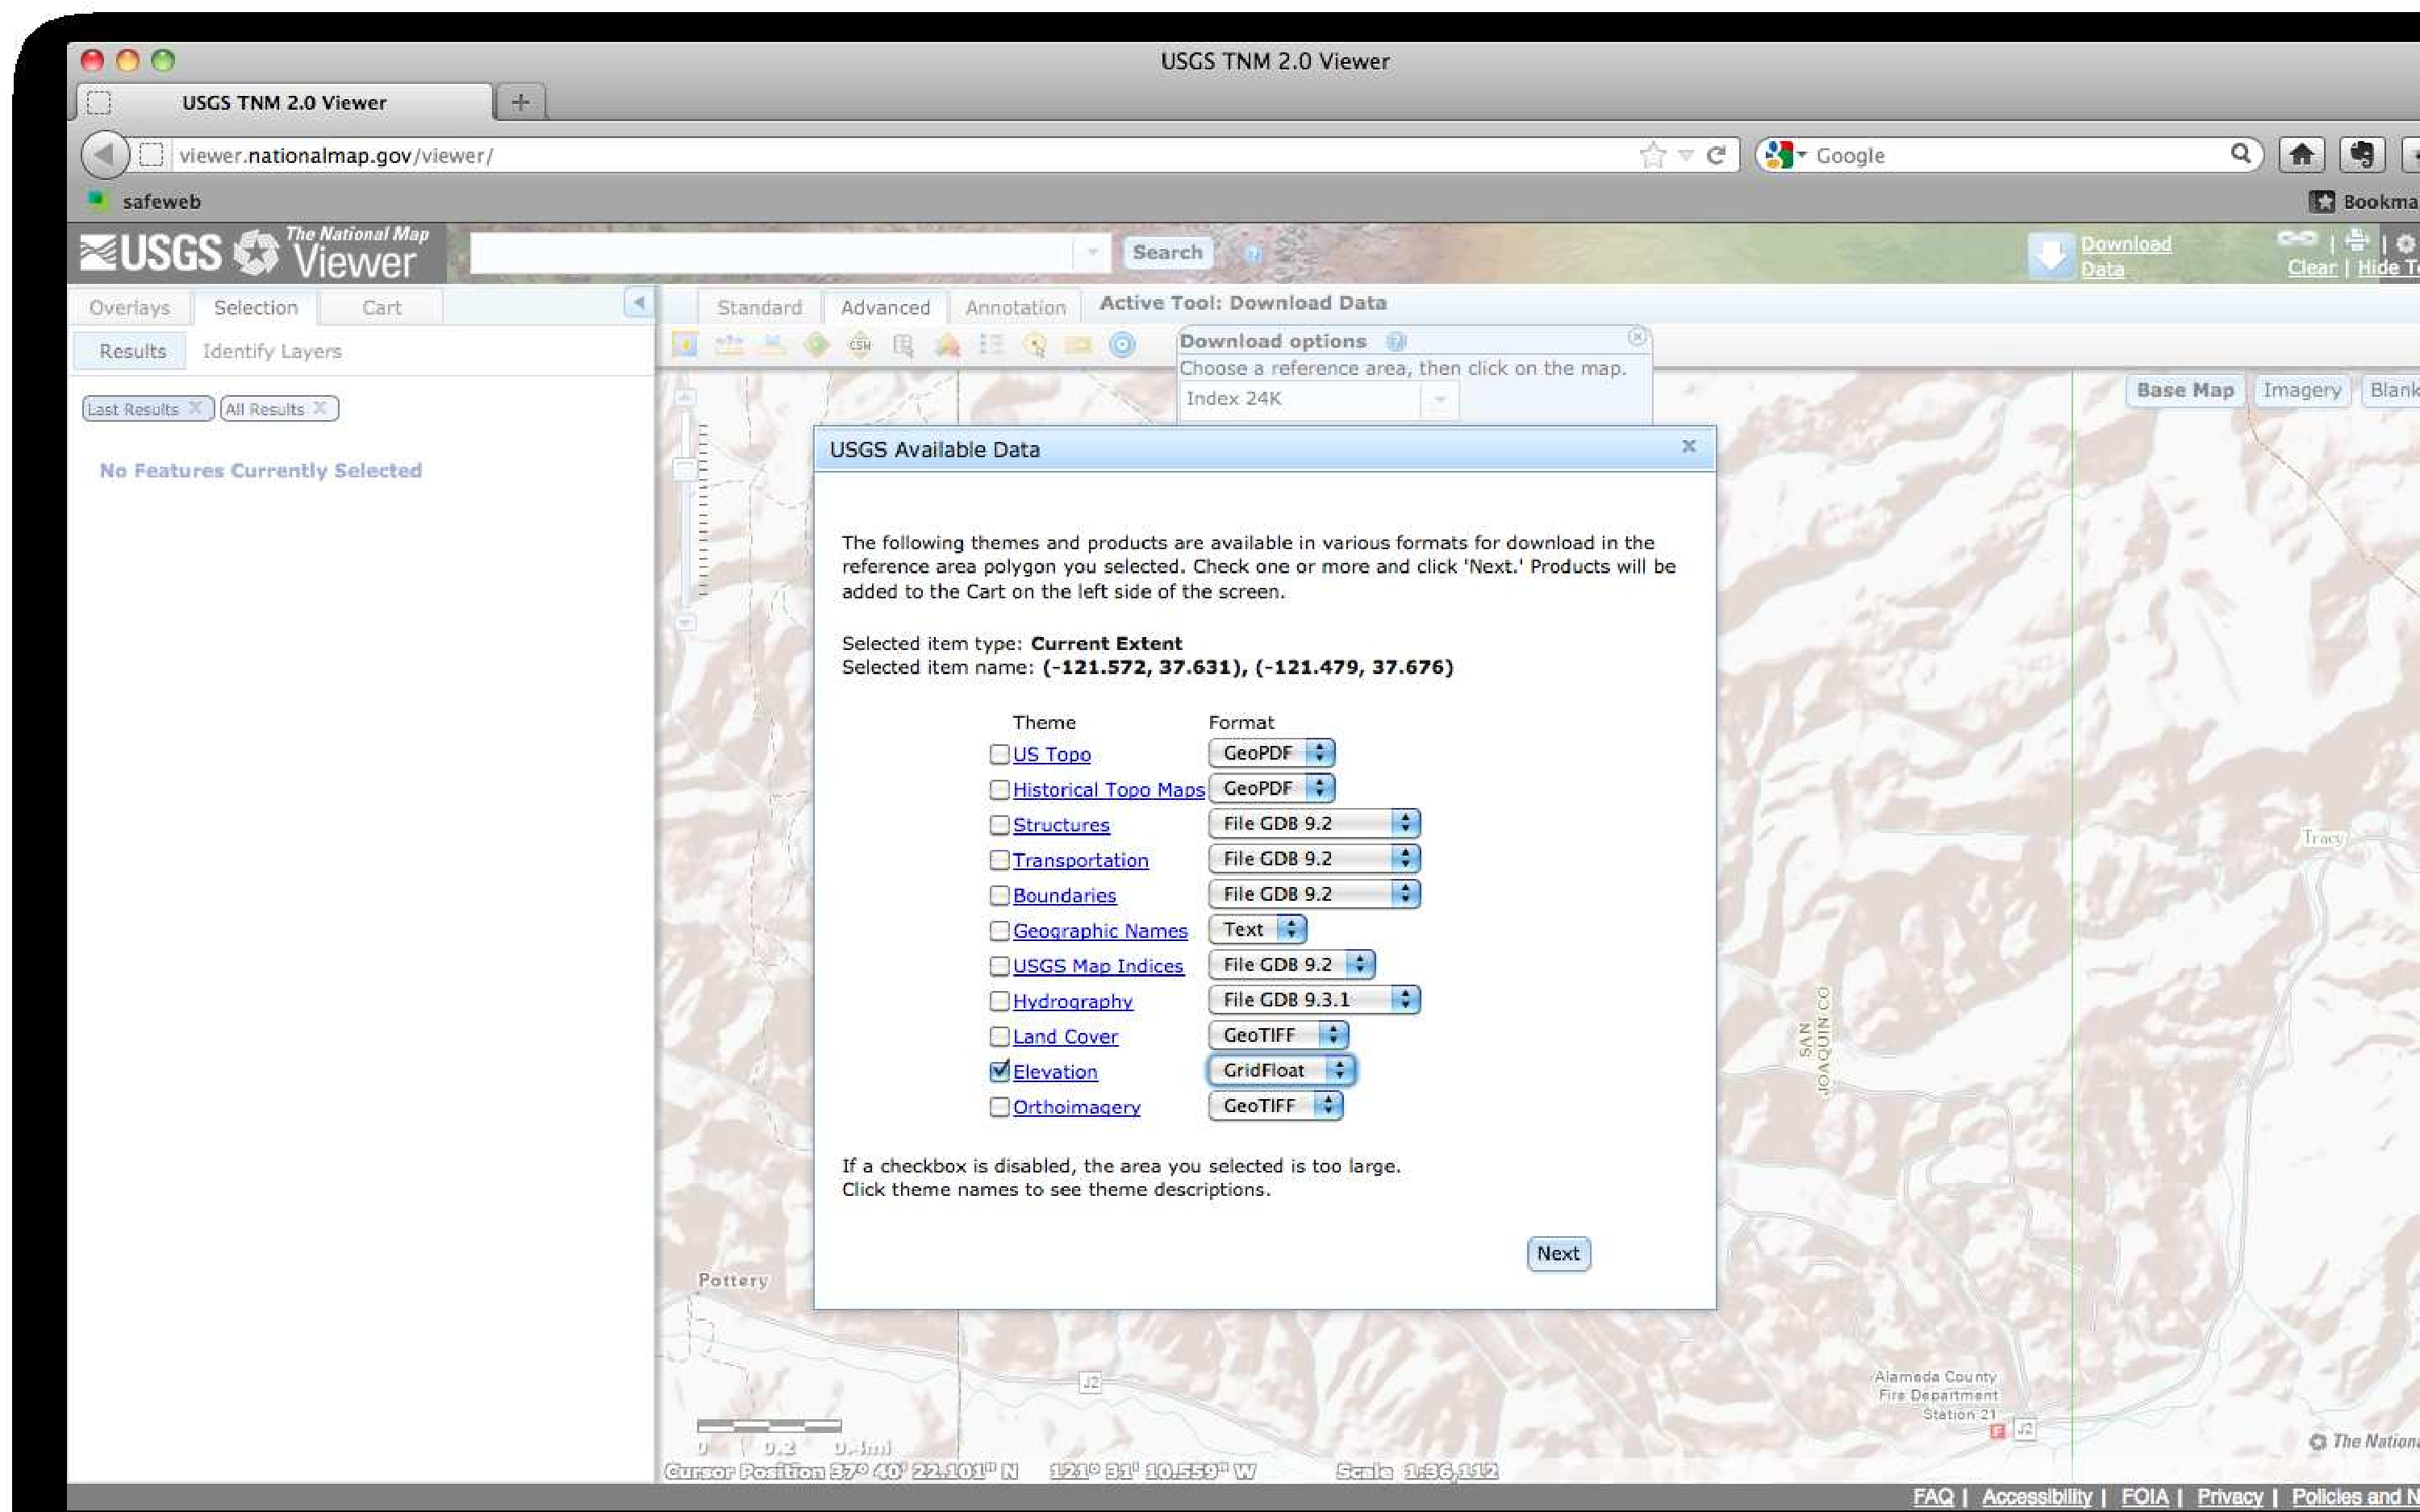
\includegraphics[width=\mapFigWidth]{fig/NationalMapFig2}
%- \par\end{centering}
%- 
%- \caption{\label{fig:Data-sets-and}Selecting a format for your data set.}
%- \end{figure}
%- 
%- \begin{figure}
%- \begin{centering}
%- 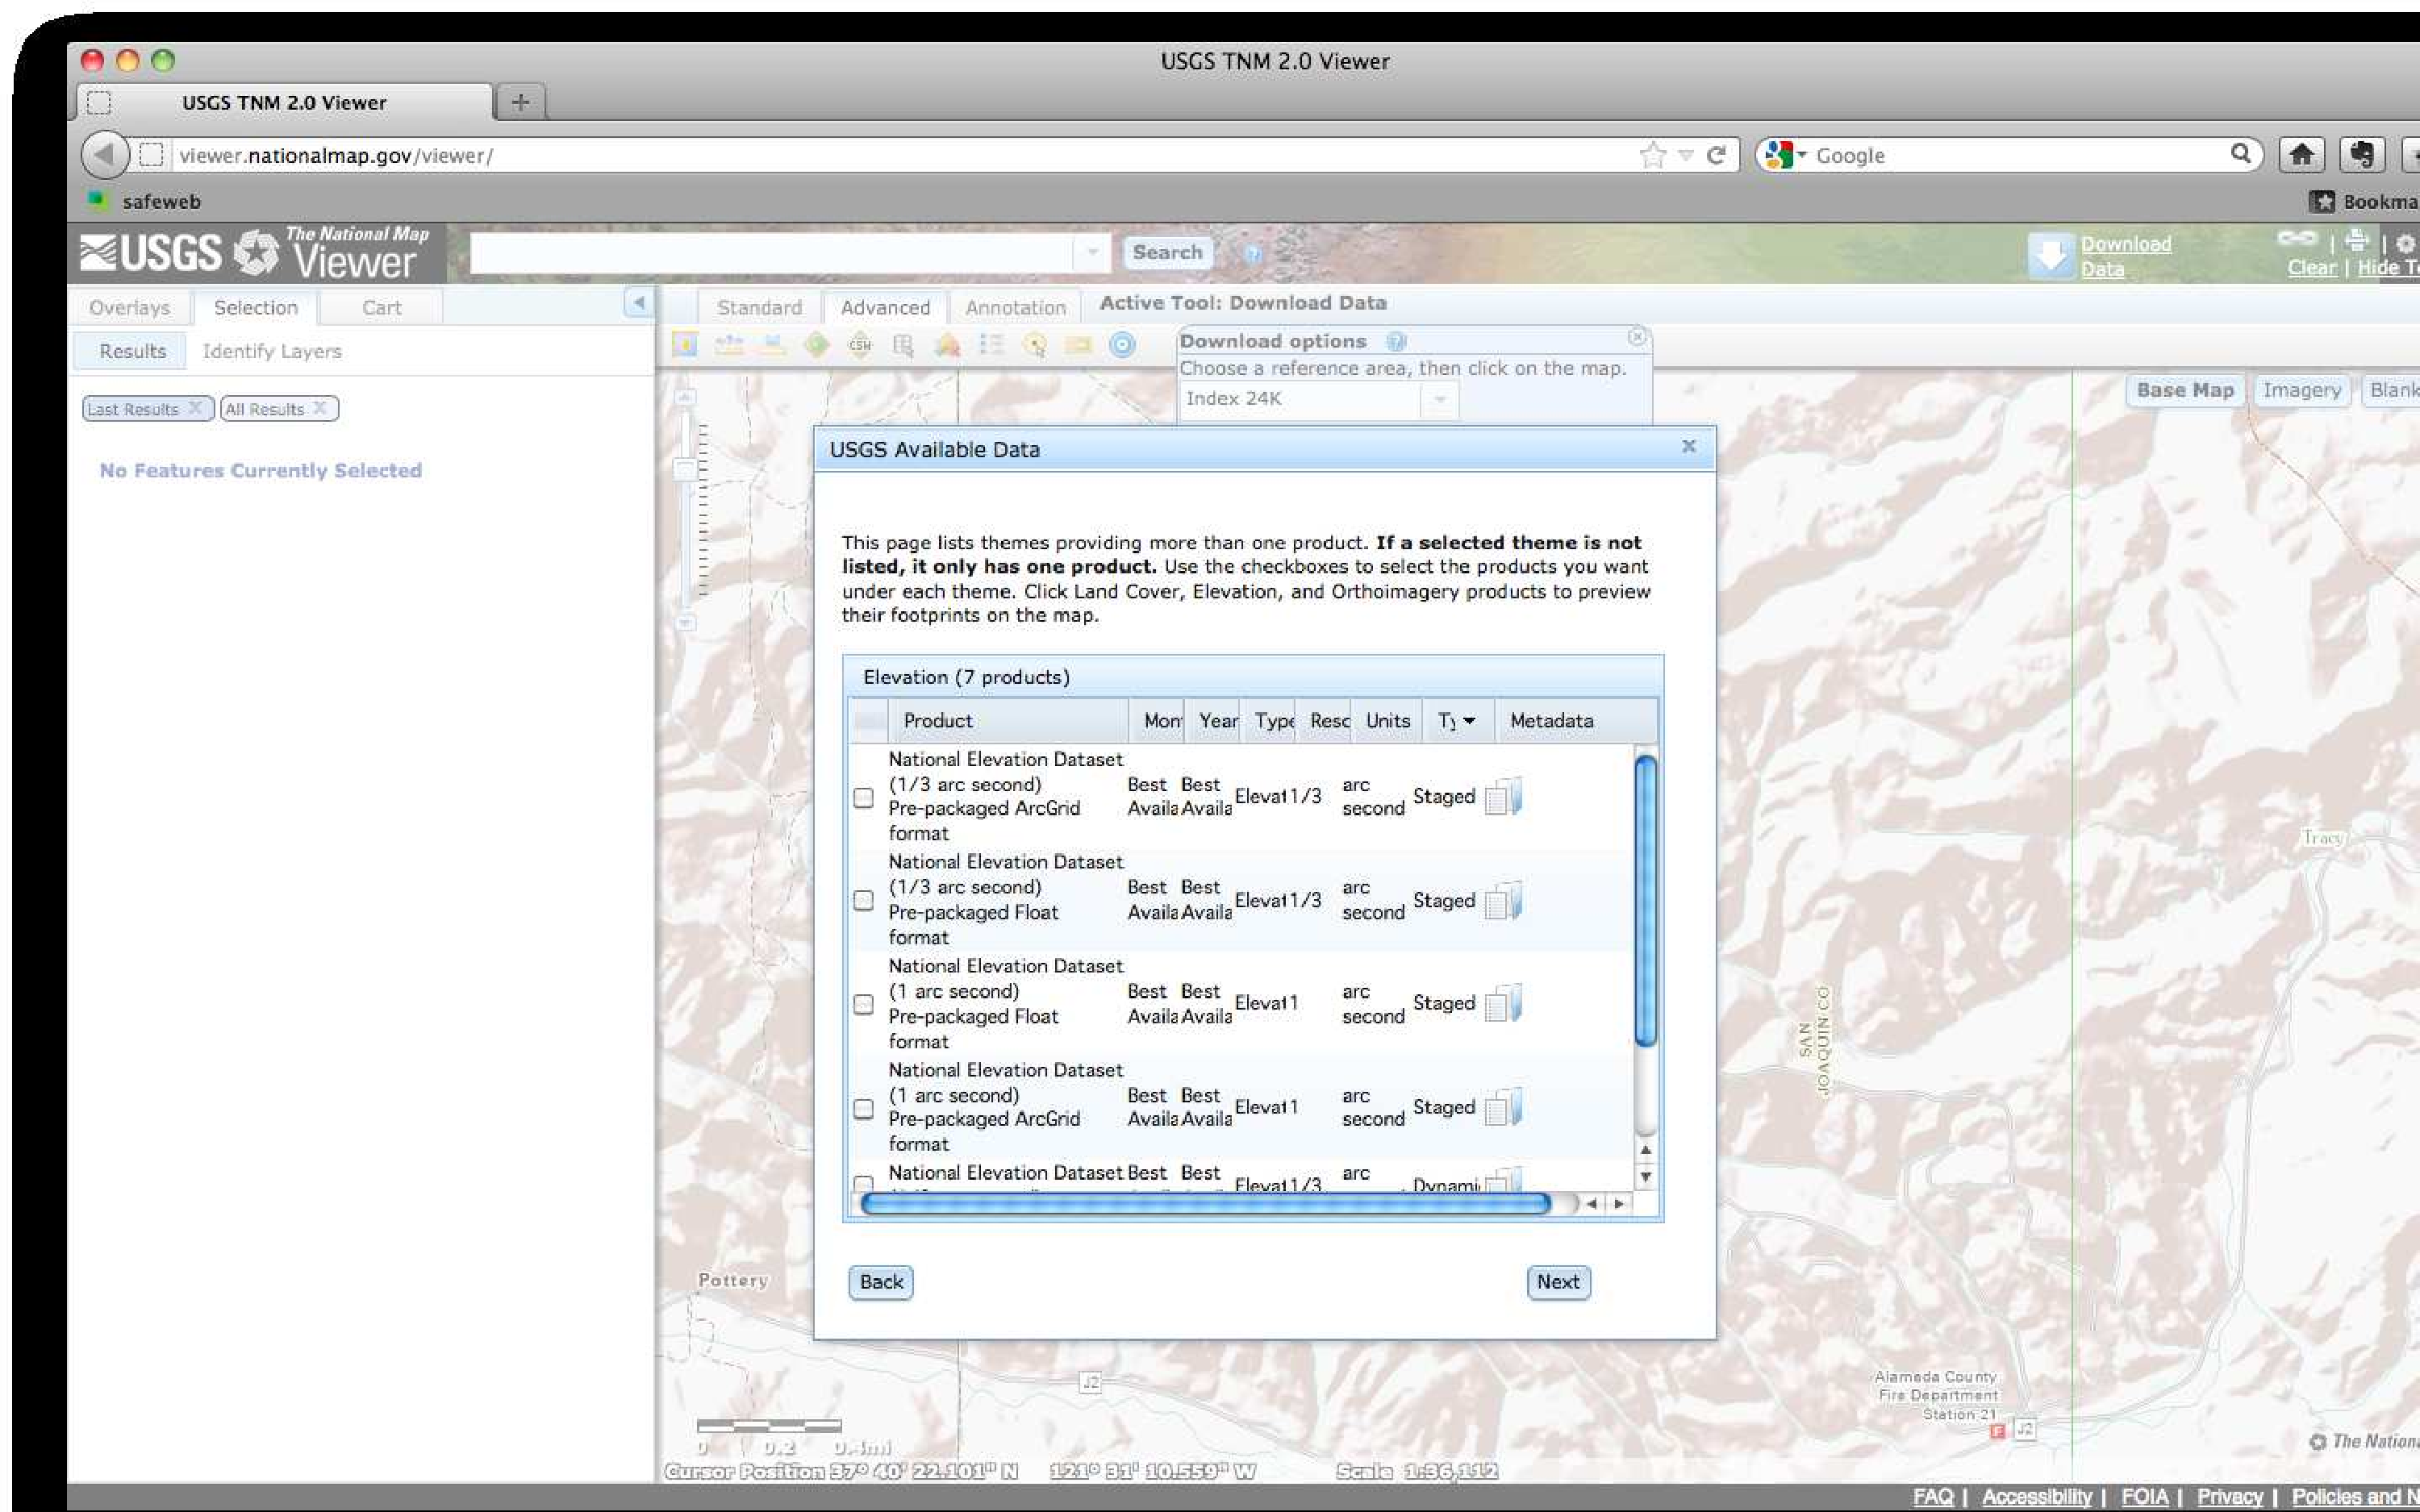
\includegraphics[width=\mapFigWidth]{fig/NationalMapFig3}
%- \par\end{centering}
%- \caption{\label{fig:Selecting-the-arcsecond}Selecting the arc second resolution
%- of your data set.}
%- \end{figure}
%- 
%- \begin{figure}
%- \begin{centering}
%- 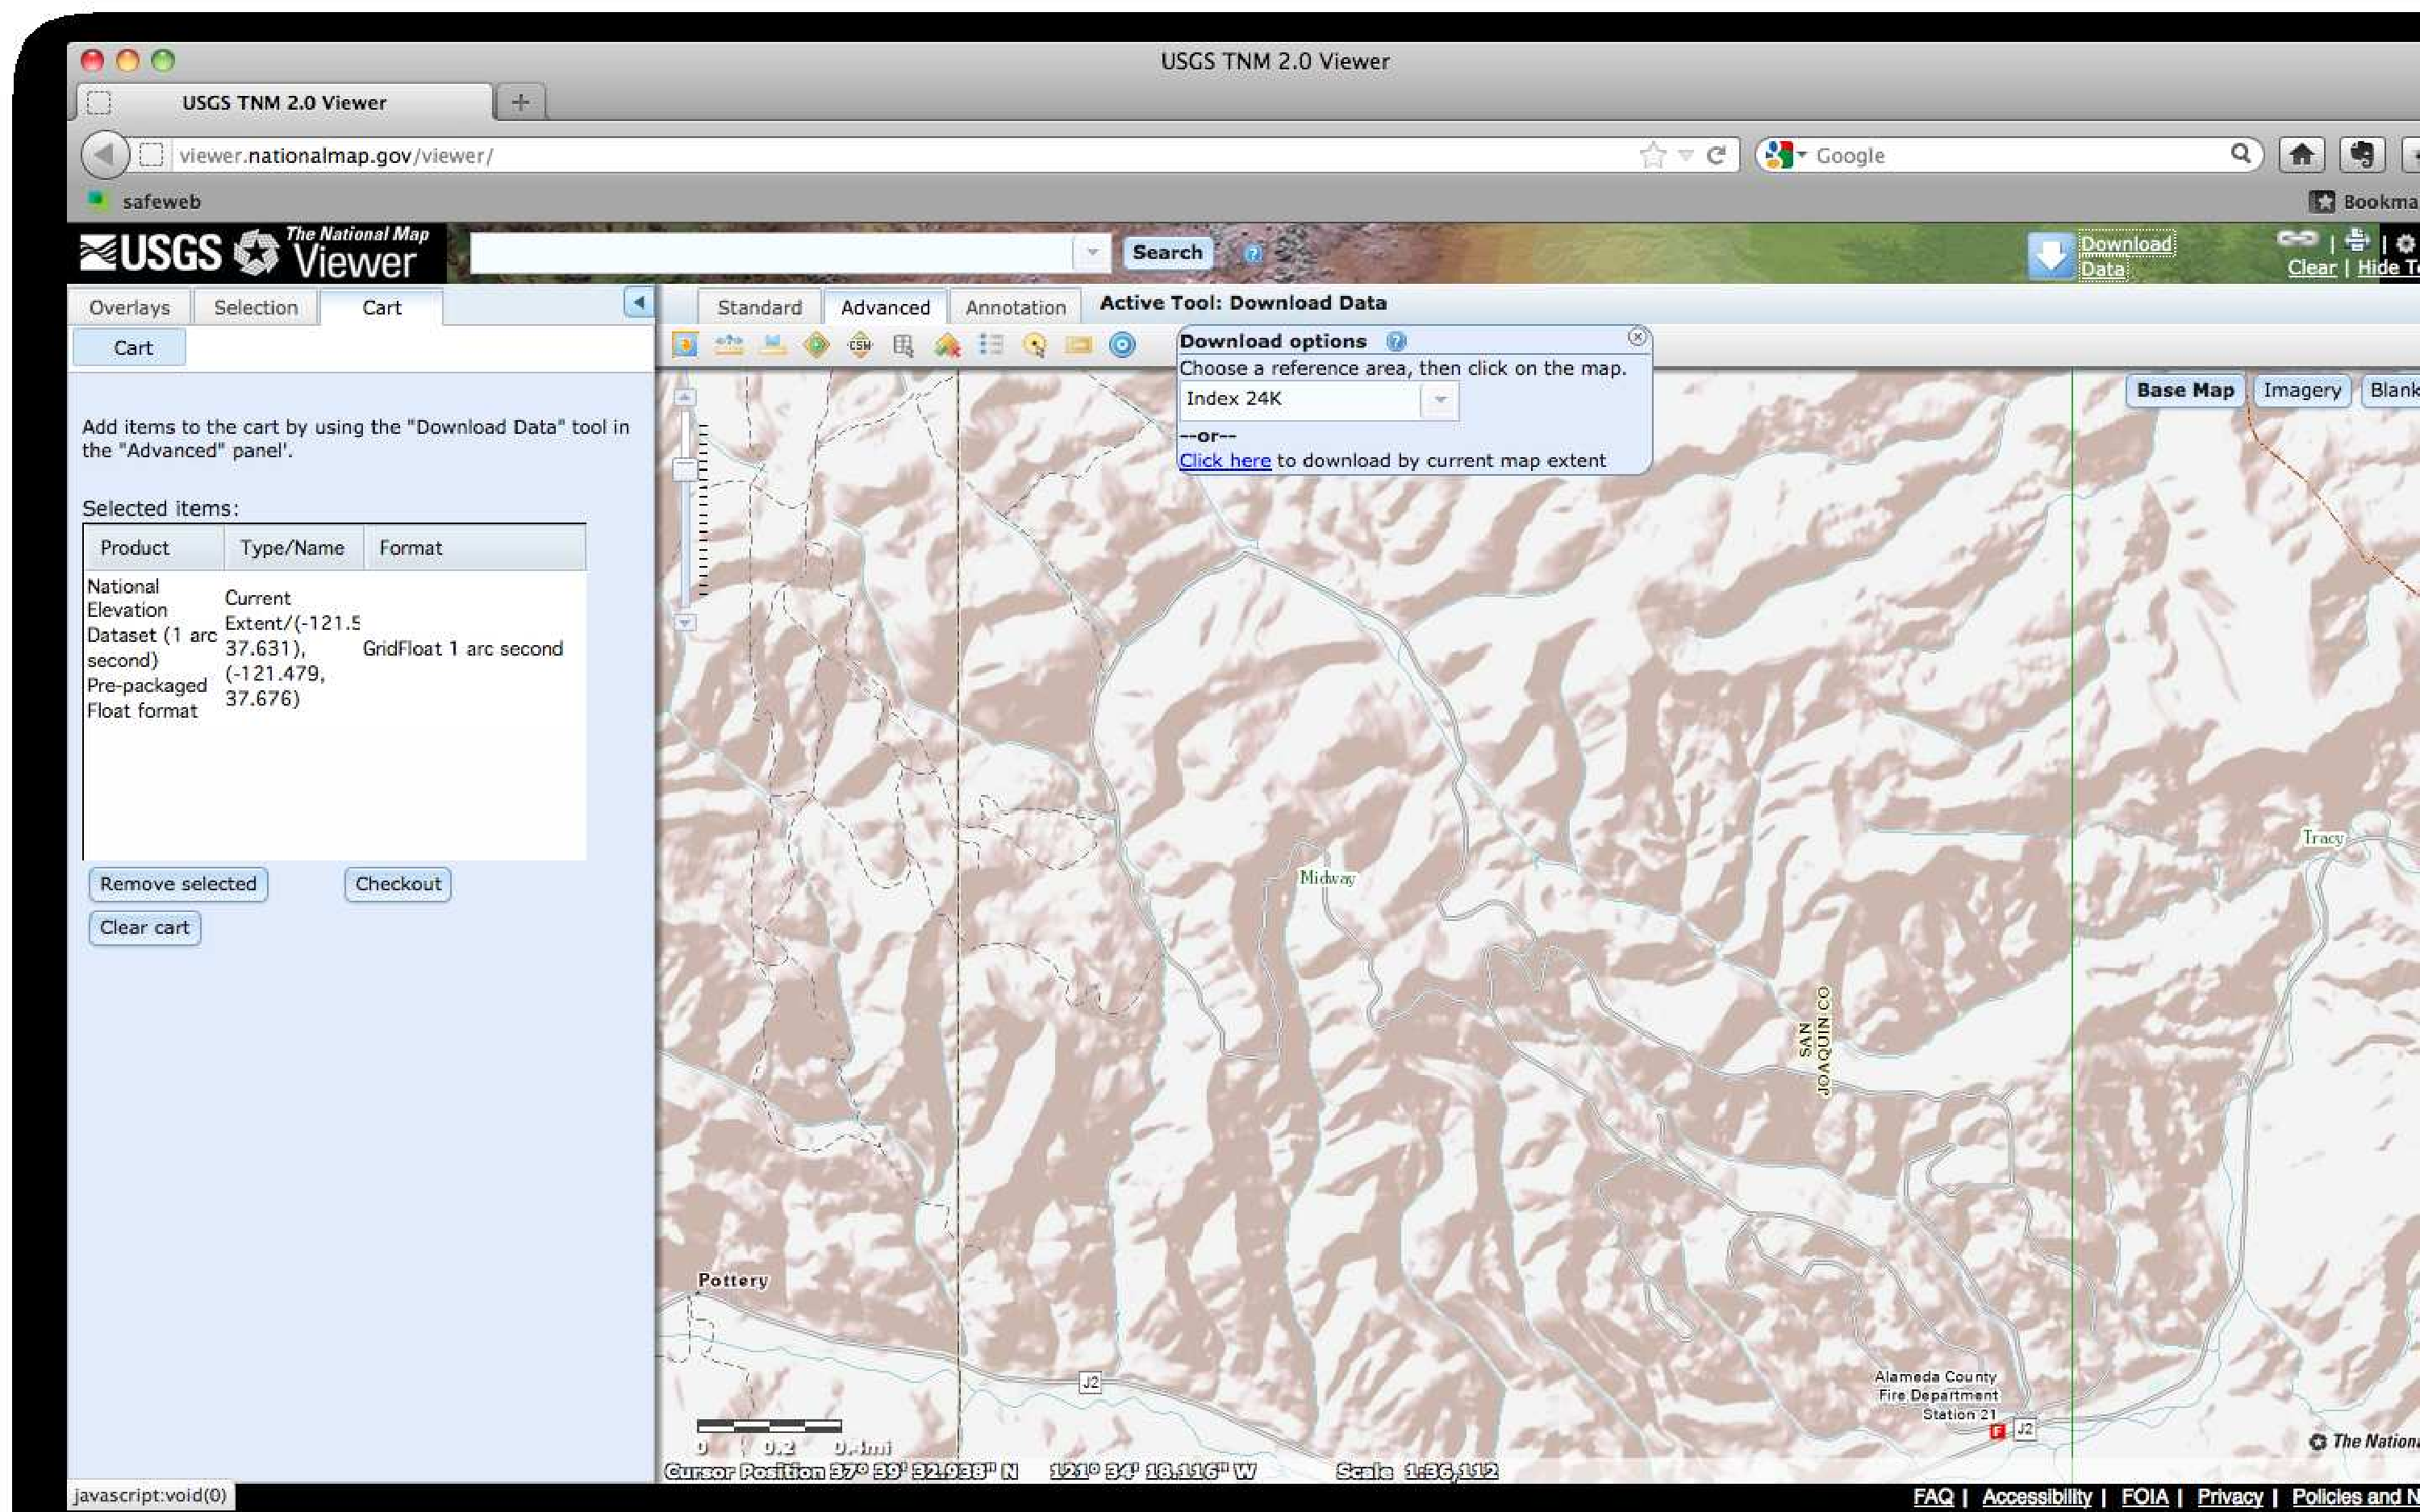
\includegraphics[width=\mapFigWidth]{fig/NationalMapFig4}
%- \par\end{centering}
%- 
%- \caption{\label{fig:The-checkout-cart.}Behold! The checkout cart.}
%- \end{figure}
%- 

%- % ================================================================================================================
%- \section{Extract GIS Data Points (USGS)}
%- 
%- 
%- \subsection{Downloading GridFloat Data from USGS}  \ref{sec:downloadGIS}
%- 
%- In order to turn USGS data into a grid for Cgins, the data must first
%- be downloaded from the USGS website, specifically the National Map
%- Viewer found at:
%- \begin{flushleft}\tt
%- http://nationalmap.gov/viewer.html 
%- \end{flushleft}
%- Using this service, particular areas on a map can be selected, and
%- geographic information downloaded. This process is covered briefly
%- here.
%- 
%- Begin by selecting a particular region of interest in the map viewer
%- (Figure \ref{fig:Region-of-interest}). The pointer shows the latitude/longitude
%- of the pointer's current location, so this can be used to obtain GIS
%- information for particular latitudes and longitudes. Once the area
%- of interest has been found and is contained in the viewport, click
%- the ``Download Data'' link in the toolbar at the top.
%- 
%- 
%- 
%- 
%- You will be presented with two choices: to either download data for
%- a reference area, or to download the current map's extent. The latter
%- can be picked by clicking the link. This will present a list of options
%- for data sets and formats (Figure \ref{fig:Data-sets-and}). The GridFloat
%- format is the desired format. Once it is downloaded, this data will
%- be processed with a Matlab script to convert it into a plain CSV file. 
%- 
%- 
%- 
%- 
%- Once you have made your selection of what dataset to download, and
%- in what format, you must also select the fineness of the data - 1
%- arc second and 1/3 arc second are available for nearly every area.
%- Note that when you select how many arc seconds you would like your
%- data to have, you must also select the correct format (as it will
%- sometimes ignore your selection of GridFloat format on the previous
%- screen).
%- 
%- 
%- 
%- 
%- The last step is to add this data to your ``cart'' and ``check
%- out'' (everything is free). Once you have done this, you will provide
%- USGS with an email address, and a link with the zip file will be emailed
%- to you.
%- 
%- 
%- 
%- % ubsection{Notes on the GridFloat Data Format}
%- 
%- The GridFloat data is contained in two files with ``flt'' and ``hdr'' (header)
%- extensions, located in the directory created when the USGS data is
%- unzipped. These files are read by the {\tt readTerrain.m} Matlab script as
%- described in Section~\ref{sec:readTerrain}
%- 
%- % The format is read in by Matlab; Matlab can be used to convert
%- % the data to a plain ASCII format, or to process the data for other uses.


% ------------------------------------------------------------------------------------------
\section{Preprocessing the NED terrain files}  \label{sec:readTerrain}
% \section{Smooth, slice or add buffer zones to the GIS terrian data (Matlab) - readTerrain.m}  \label{sec:readTerrain}

The Matlab script {\tt readTerrain.m} (found in {\tt cg/ins/runs/terrain})
reads the NED (National Elevation Dataset) terrain files that were obtained from the USGS web site (Section~\ref{sec:NationalMapViewer})
and generates the files that are needed for generating an overlapping grid with Ogen. The {\tt readTerrain.m}
script can be used to
\begin{enumerate}
  \item extract a sub-domain, 
  \item extract a cross-section for a two-dimensional simulation,
  \item smooth the terrain data,
  \item add buffer zones around the terrain region.
\end{enumerate}
See the comments at the top of the {\tt readTerrain.m} script to see the various options.

Figure~\ref{fig:AltamontPass} shows the surface created from a NED file for the region near
the Altamont Pass in California. The data files for this region, {\tt AltamontPass.hdr} and
{\tt AltamontPass.flt}, are found in {\tt cg/ins/runs/terrain}. The region is centered near $(-121.643519^o,37.724444^o)$ 
 (longitude $121^o~38'~36.6"$ W and latitude $37^o~43'~27.84"$ N) and the surface
was created with the command, 
\begin{flushleft}\tt
  readTerrain -file=AltamontPass -name=AltamontPass -plotOption=1 -long0=-121.643519 -lat0=37.724444 -xWidth=3000 -yWidth=3000
\end{flushleft}
% Here is an example matlab command that can be used:
% \begin{flushleft}\tt
%   readTerrain -file=AltamontPass -name=AltamontPass -plotOption=1 -long0=-121.643519 -lat0=37.724444 -xWidth=3000 -yWidth=3000
% \end{flushleft}
% \begin{flushleft}\tt
%    readTerrain -file=NED\textunderscore81691785/ned\textunderscore1691785 -name=SanFrancisco -long0=-122.4785 -lat0=37.819471 -xWidth=5000 -yWidth=-5000 
% \end{flushleft}
In this case we have selected a region of size $3000m\times 3000m$ centered at a longitude of $-121.643519^o$ and 
latitude of $37.724444^o$. 

In later sections we will consider the flow over the terrain in a part of LLNL's {\em Site 300} property (see Figure~\ref{fig:site300Terrain}).
The NED data files for this region are {\tt site300.hdr} and {\tt site300.flt} and are found 
in the directory {\tt cg/ins/runs/terrain}. Here is the Matlab command to create {\tt site300.dat}, 
\begin{flushleft}\tt
  readTerrain -file=site300 -name=site300 -plotOption=2 -smooth=1 -yCrossSection=725 -xCrossSection=600
\end{flushleft}

Note that {\tt readTerrain.m} converts the lat-long coordinates from the NED file into meters. This is done
using a formula for the arclength between two points on a sphere  (known as the haversine formula, see wikipedia)
\begin{align*}
   \xv_{i,j} = 2 R_{\rm earth} \sin^{-1}\Big( \sqrt{ \sin^2(( \phi_j - \phi_0 )/2) + \cos(\phi_0)\cos(\phi_j) \sin^2((\lambda_i-\lambda_0)/2) } \Big),
\end{align*}
where $R_{\rm earth}=6.3781\times 10^6 m$ is the radius of the earth, $(\lambda_0,\phi_0)$ are the long-lat coordinates (in radians) of the
lower left corner of the region and $(\lambda_i,\phi_j)$ are the long-lat coordinates of grid point $(i,j)$.
{\bf Note 1:} the haversine formula is well conditioned for small distances but has troubles near the poles.
{\bf Note 2:} that there is some approximation made in this formula since we are projecting the sphere onto a plane. This
approximation should be good if the region is only a few kilometers wide.

As noted, the {\tt readTerrain.m} script can select a sub-domain of the entire terrain data based on a latitude/longitude
location and a bounding box. 
The selected elevation data may be smoothed (this is recommended)
using a fourth-order filter in the interior and a second-order filter near the boundary. The extra smoothing near
the boundary is done to make the surface more or less horizontal near the boundary. 
This makes it easier to generate a volume grid where the grid lines on the edges are vertical and thus match
to the Cartesian background grids. 
The terrain data, before and after smoothing, can
be plotted from using {\tt readTerrain.m}. Usually the smoothed terrain is nearly indistinguishable from the
orginal data in the interior of the domain, while the boundary regions have clearly been smoothed. 

The terrain data can also optionally be sliced along a constant value of $x$ or $y$ in order to generate
a two dimensional curve for use in two-dimensional Cgins simulations. It is highly recommended that one first
perform some two-dimensional calculations in order to get a familiar with Cgins and the various options.


Once the data have been manipulated as
desired, they are saved to a data file (e.g. named {\tt AltamontPass.dat} for the command above, {\tt -name=AltamontPass}). 
This file is read by the Ogen script {\tt terrainGrid.cmd} (see Section~\ref{sec:terrainGridGeneration})
to generate an overlapping grid. The data in the file actually defines points on a surface that
are used to construct a NURBS (Non-Uniform Rational B-Spline).





{%%%
\newcommand{\figWidtha}{11.cm}
\newcommand{\trimfiga}[2]{\trimPlot{#1}{#2}{.0}{.0}{.0}{.0}}
\newcommand{\figWidthb}{7.cm}
\newcommand{\trimfigb}[2]{\trimPlot{#1}{#2}{.15}{.175}{.4}{.3}}
% 
% % -----------------------------------------------------------------------------------------------------------------------------------------
\begin{figure}[hbt]
\begin{center}
\begin{tikzpicture}[scale=1]
  \useasboundingbox (0,.5) rectangle (18.,6.5);  % set the bounding box (so we have less surrounding white space)
%
\draw (0.0,0.0)  node[anchor=south west,xshift=-4pt,yshift=+0pt] {\trimfiga{fig/AltamontPassOriginal}{\figWidtha}};
% draw a box around the region
\begin{scope}[xshift=11cm]
  \draw (0,0.0)  node[anchor=south west,xshift=-4pt,yshift=+0pt] {\trimfigb{fig/AltamontPassTopo}{\figWidthb}};
  \draw[line width=2pt] (2.2,2.2) -- (4.6,2.2) -- (4.6,4.6) -- (2.2,4.6) -- (2.2,2.2);
\end{scope}
%
% \draw[step=1cm,gray] (0,0) grid (18,6.);
\end{tikzpicture}
\end{center}
 \caption{Terrain near the Altamont Pass, CA. Left, surface from {\tt readTerrain.m}. Right: topographic map. The terrain
   on the left corresponds roughly to the region outlined on the right.}
  \label{fig:AltamontPass}
\end{figure}
% -----------------------------------------------------------------------------------------------------------------------------------------------
%
}%

Buffer regions can be extended from the terrain region in selected directions in order to provide a smooth terrain profile near the
boundaries of the computational region, see Figure~\ref{fig:terrainSmoothBuffer}. 
A buffer zone may be needed at outflow boundaries to prevent strong
recirculation regions (from steep terrain near the outflow) from hitting the outflow boundary and 
causing a locally strong inflow condition that may cause difficulties in the flow solver. The Cgins flow solver
has an option {\tt expect inflow at outflow} that can be used at outflow boundaries and with this option buffer
zones may not be needed. 


%- The final output of the Matlab script is a three-dimensional surface;
%- an example can be found in the following file:
%- \begin{flushleft}\tt
%-     cg/ins/runs/terrain/site300Full.dat
%- \end{flushleft}
%- The file is formatted in such a way that a nurbs (non-uniform rational
%- B-spline) map can be created from it. The nurbs map is created by
%- ogen, the CGINS grid generator tool, which reads in the data file
%- created by readTerrain.m.


{%%%
\newcommand{\figWidthb}{9.cm}
\newcommand{\trimfigb}[2]{\trimPlot{#1}{#2}{.0}{.0}{.0}{.0}}
% 
% % -----------------------------------------------------------------------------------------------------------------------------------------
\begin{figure}[hbt]
\begin{center}
\begin{tikzpicture}[scale=1]
  \useasboundingbox (0,.5) rectangle (18.,5.5);  % set the bounding box (so we have less surrounding white space)
%
\draw (0.0,0.0)  node[anchor=south west,xshift=-4pt,yshift=+0pt] {\trimfigb{fig/site300WithBufferOriginal}{\figWidthb}};
\draw (9.0,0.0)  node[anchor=south west,xshift=-4pt,yshift=+0pt] {\trimfigb{fig/site300WithBufferSmoothed}{\figWidthb}};
%

% \draw (current bounding box.south west) rectangle (current bounding box.north east);
% grid:
% \draw[step=1cm,gray] (0,0) grid (18,5.5);
\end{tikzpicture}
\end{center}
 \caption{The {\tt readTerrain.m} Matlab script can be used to add buffer zones and smooth the elevation data.
Top: original terrain data with buffer zones added (The buffer zones are 20 grid points wide on three sides and
   50 grid points wide on the fourth side). Bottom: smoothed terrain data.}
  \label{fig:terrainSmoothBuffer}
\end{figure}
% -----------------------------------------------------------------------------------------------------------------------------------------------
%
}%

\section{Generating an overlapping grid with Ogen} \label{sec:terrainGridGeneration}

Ogen is Overture's overlapping grid generator and is used to cut holes and determine interpolation
points~\cite{OGEN}.
The Ogen command file {\tt terrainGrid.cmd} can be used to generate a three-dimensional
overlapping grid for a region above the terrain.   
Here is an example command that generates a grid:
\begin{flushleft}\tt
   ogen -noplot terrainGrid -interp=e -site=site300.dat -prefix=site300  -topLevel=700 -order=4 -factor=4 -ml=2
\end{flushleft}
This example generates a fourth-order accurate (-order=4) grid with explicit interpolation (-interp=e) with a target horizontal grid
spacing of $20/4=5$ m (-factor=4) with two multigrid levels (-ml=2). The grid extends in the vertical direction to a height
of $700m$ (-topLevel=700) above the lowest point on the terrain. 
See the comments at the top of {\tt terrainGrid.cmd} for a full description of the options.

Here are some more details on the grid:
\begin{itemize}
   \item The data file (e.g. {\tt site300.dat}) generated from {\tt readTerrain.m} (see Section~\ref{sec:readTerrain}) is included
   in the Ogen script {\tt terrainGrid.cmd}. 
   Note that this data file contains the bounds of the grid in the $x$ and $y$ directions (used to dimension the background grids), 
   in addition to the data points that define the NURBS surface. 
   \item The basic overlapping grid for the terrain consist of a surface-fitted 
     curvilinear grid near the ground surface, a refined Cartesian background grid near
     the surface (by default extending to a height {\tt -midLevel=300} above the lowest point on the terrain), 
     and a coarsened background grid that extends upward to a height specified by {\tt -topLevel}.
     A two-dimensional terrain grid is shown in Figure~\ref{fig:site300Grid2d}, while a three-dimensional grid
     is shown in Figure~\ref{fig:site300Grid}.
     The curvilinear grid near the surface is stretched in the normal direction to decrease the spacing near the ground.
\end{itemize}





% \section{Create a Nurbs Map (ogen)}
% 
% Once the Matlab script has been run, the full three-dimensional surface
% can be included in an ogen script, such as the ogen script located
% at:
% \begin{flushleft}\tt
% \textasciitilde{}reid24/for\_all/site300Grid.cmd
% \end{flushleft}
% The ogen script converts the output of the Matlab file into a nurbs
% map; the output of the Matlab file contains information about the
% minimum and maximum values in each direction. The nurbs map is then
% used to create a composite grid with specified parameters (order,
% length scale, levels, overlap factor, etc.). The nurbs mapping is
% parametrically a two dimensional square (domain dimension 2) mapped
% to a physical volume in three dimensions (range dimension 3).
% 
% The hyperbolic grid generator extends each grid several extra points
% out into the domain, and uses these extra points to match with the
% background grid and get a composite grid. At the time that the grid
% is generated, ogen must know the order of accuracy of the solution
% technique, so that it knows the stencil size and corresponding amount
% of overlap each grid needs. The grid generator assumes a ``worst
% case scenario'' with respect to stencil size - that is, that stencils
% are not sparse.
% 
% To run a cmd file using ogen, first set the CGWIND environmental variable
% to point to your CGINS binary, then execute the ogen command. This
% can be done as follows:
% \begin{flushleft}\tt
% ogen -noplot terrainGrid.cmd -interp=e~-order=2~-factor=4~-ml=2
% \end{flushleft}
% where -interp=e means use explicit interpolation for the overlapping
% regions of the grid, -order=2 means generate grids that have enough
% ghost points to be used with a second order scheme, -factor=2 means
% use a grid stretching factor of 4, and -ml=2 means 2 levels for the
% multi-level solver.
% 
% This command will generate a grid, which will have an extension of
% hdf. This grid can be visualized using plotStuff:
% \begin{flushleft}\tt
% /plotStuff~site300Grid2de4.order2.ml2.hdf
% \end{flushleft}
% and will look like the window shown in Figure \ref{fig:plotStuff}.
% Alternatively, once a sequence of commands has been performed in plotStuff,
% that sequence of commands will be saved to a command file (with file
% extension .cmd), which can then be applied to other grids to perform
% the same sequence of commands and obtain similar resulting plots. 
% 
% \begin{comment}
% {[}hole-cutting: determining where the mask is (also good for debugging,
% in case you improperly indicate the domain){]}
% \end{comment}
% 
% 
% \begin{figure}
% \begin{centering}
% \includegraphics[scale=0.2]{fig/plotStuff1}
% \par\end{centering}
% 
% \caption{\label{fig:plotStuff}A sample (two-dimensional) grid of Site 300
% created using GIS data and a Nurbs map, and plotted using the plotStuff
% tool.}
% \end{figure}
% 
% 
% \begin{figure}
% \begin{centering}
% \includegraphics[scale=0.2]{fig/plotStuff2}
% \par\end{centering}
% 
% \caption{\label{fig:plotStuffZoomed}Zoomed-in view of two-dimensional overlapping
% grids, with interpolation points (square black dots) plotted.}
% 
% 
% \end{figure}
% 
% 
% \begin{figure}
% \begin{centering}
% \includegraphics[scale=0.4]{fig/plotStuffOptions}
% \par\end{centering}
% 
% \caption{\label{fig:plotStuffOptions}A subwindow containing a range of options
% available in plotStuff. The ``Plot interpolation points'' option
% adds the black interpolation points seen in Figure \ref{fig:plotStuffZoomed}.}
% 
% 
% \end{figure}
% 


%- \section{Running the Flow Solver (Cgins)}
%- 
%- 
%- \subsection{Running in Serial}
%- 
%- Once the grid is satisfactory, running CGINS/CGWind is the next step.
%- To do this, the CG directory must be set using the CG environmental
%- variable:
%- \begin{flushleft}\tt
%- export~CG=/g/g10/henshaw/cg
%- \end{flushleft}
%- Next, the cgins binary is invoked, pointed to the ogen .cmd file to
%- be used (site3002d.cmd, with the file extension omitted), pointed
%- to the grid .hdf file to be used (site300Gride4.order2.ml2.hdf, with
%- the file extension omitted), and its various options set:
%- \begin{flushleft}\tt
%- /usr/gapps/overture/cg.ga/ins/bin/cgins~\textbackslash{}
%- 
%- ~~~~\textasciitilde{}reid24/for\_all/site300run~\textbackslash{}
%- 
%- ~~~~-g=site300Gride4.order2.ml2~-nu=1.~\textbackslash{}
%- 
%- ~~~~-ad2=1~-ts=afs~-cfl=6.~-slowStartCFL=2.~\textbackslash{}
%- 
%- ~~~~-slowStartSteps=100~-slowStartRecomputeDt=10~-recomputeDt=50~\textbackslash{}
%- 
%- ~~~~-tp=5.~-ts=afs~-psolver=mg~-debug=1
%- \end{flushleft}
%- (Alternately, the command-line options given above can be left out,
%- and the values specified in the .cmd file will be used instead). This
%- command will run cgins in serial mode.
%- 
%- \begin{figure}
%- \begin{centering}
%- \includegraphics[scale=0.25]{fig/cginsSerial1}
%- \par\end{centering}
%- 
%- \caption{\label{fig:cgwindSerial}Plotting results of a timestep from a serial
%- run of cgins.}
%- 
%- 
%- \end{figure}


% ========================================================================================================
% \clearpage
\newcommand{\Gt}{\Gc_{t}}
\section{Simulating the flow over terrain using Cgins}\label{sec:terrain}


The commands used to run the examples in this Section can be found in {\tt cg/ins/runs/terrain/Readme}.


% \newcommand{\ds}{\Delta s}
\newcommand{\dsj}{\ds^{(j)}}
% ---------------------------------------------------------------------------------------------
\subsection{Two dimensional computations}

We start by first performing some two-dimensional computations. We choose a cross-section through
the three-dimensional data. This curve in shown in Figure~\ref{fig:site300Terrain}.
The two-dimensional grid is shown in Figure~\ref{fig:site300Grid2d}.
Let $\Gc^{(j)}$ denote the overlapping grid for this domain with a target grid spacing of $\dsj=20/j$. 
A narrow curvilinear {\em terrain} grid is located next to the terrain surface. This grid is stretched in
the normal direction. A fine Cartesian grid is located above the surface. The grid resolution of this
grid is $\dsj$ and matches that of the outer spacing on the terrain grid. A coarser back-ground grid is placed above both
these grids with grid spacing $\dsj \times 2$. The upper elevation of this grid is at $700$m above the lowest point on
the terrain.


{
\begin{figure}[hbt]
\newcommand{\figWidth}{13cm}
\newcommand{\trimfig}[2]{\trimFig{#1}{#2}{0.025}{.025}{.25}{.25}}
\newcommand{\figWidtha}{7cm}
\newcommand{\trimfiga}[2]{\trimFigb{#1}{#2}{0.0}{.0}{.5}{.1}}
\begin{center}\small
% ------------------------------------------------------------------------------------------------
\begin{tikzpicture}[scale=1]
  \useasboundingbox (0,0.25) rectangle (14,7.);  % set the bounding box (so we have less surrounding white space)
  \draw ( 0, 0) node[anchor=south west,xshift=-4pt,yshift=-4pt] {\trimfig{fig/site300Grid2dO2G4}{\figWidth}};
  \draw (7, 2.5) node[anchor=south west,xshift=-4pt,yshift=-4pt] {\trimfiga{fig/site300Grid2dO2G4Zoom}{\figWidtha}};
%  \draw[step=1cm,gray] (0,0) grid (14,8);
\end{tikzpicture}
% ----------------------------------------------------------------------------------------
\caption{Two-dimensional overlapping grid for a cross-section through the terrain. Grid $\Gc^{(4)}$ (second-order accuracy) is shown
   along with a magnified view of the grid near the surface.}
\label{fig:site300Grid2d}
\end{center}
\end{figure}
}

Figure~\ref{fig:site300Flow2d} shows results for different grid resolutions and different orders of accuracy.
The velocity at inflow was specified as a parbolic profile (over a height of $50$m) with a maximum value
of $10m/s$ ($22.4 mph$). Since we are 
using an LES model, finer grids will have finer features. The fourth-order accurate results (AF24) are seen to generate
much finer scale features and to have less dissipation.

% ------------------- NEW ------------
{
\begin{figure}[hbt]
\newcommand{\figWidth}{8.75cm}
\newcommand{\trimfig}[2]{\trimFigb{#1}{#2}{0.025}{.025}{.2}{.45}}
\begin{center}\small
% ------------------------------------------------------------------------------------------------
\begin{tikzpicture}[scale=1]
  \useasboundingbox (0,0.7) rectangle (18,19.5);  % set the bounding box (so we have less surrounding white space)
%
  \begin{scope}[yshift=15.cm]
    \draw ( 0, 0) node[anchor=south west,xshift=-4pt,yshift=-4pt] {\trimfig{fig/site3002dO2G4slT300}{\figWidth}};
    \draw ( 9, 0) node[anchor=south west,xshift=-4pt,yshift=-4pt] {\trimfig{fig/site3002dO2G4vorT300}{\figWidth}};
    \draw (9,0.0) node[draw,fill=white,anchor=south,xshift=0pt,yshift=-2pt] {\scriptsize AFS22, $\Gc^{(4)}$, $t=300$ (second-order, coarse)};
  \end{scope}
%
  \begin{scope}[yshift=10.cm]
    \draw ( 0, 0) node[anchor=south west,xshift=-4pt,yshift=-4pt] {\trimfig{fig/site3002dO2G8slT300}{\figWidth}};
    \draw ( 9, 0) node[anchor=south west,xshift=-4pt,yshift=-4pt] {\trimfig{fig/site3002dO2G8vorT300}{\figWidth}};
    \draw (9,0.0) node[draw,fill=white,anchor=south,xshift=0pt,yshift=-2pt] {\scriptsize AFS22, $\Gc^{(8)}$, $t=300$ (second-order, fine)};
  \end{scope}
%
%
  \begin{scope}[yshift=5.0cm]
    \draw ( 0, 0) node[anchor=south west,xshift=-4pt,yshift=-4pt] {\trimfig{fig/site3002dO4G4slT300}{\figWidth}};
    \draw ( 9, 0) node[anchor=south west,xshift=-4pt,yshift=-4pt] {\trimfig{fig/site3002dO4G4vorT300}{\figWidth}};
    \draw (9,0.0) node[draw,fill=white,anchor=south,xshift=0pt,yshift=-2pt] {\scriptsize AFS42, $\Gc^{(4)}$, $t=300$ (fourth-order, coarse)};
  \end{scope}
%
  \begin{scope}[yshift=0.0cm]
    \draw ( 0, 0) node[anchor=south west,xshift=-4pt,yshift=-4pt] {\trimfig{fig/site3002dO4G8slT300}{\figWidth}};
    \draw ( 9, 0) node[anchor=south west,xshift=-4pt,yshift=-4pt] {\trimfig{fig/site3002dO4G8vorT300}{\figWidth}};
    \draw ( 9,0.0) node[draw,fill=white,anchor=south,xshift=0pt,yshift=-2pt] {\scriptsize AFS42, $\Gc^{(8)}$, $t=300$ (fourth-order, fine)};
  \end{scope}
% \draw[step=1cm,gray] (0,0) grid (18,19.);
\end{tikzpicture}
% ----------------------------------------------------------------------------------------
\caption{Computed solution for the two-dimensional domain. Streamlines and contours of the vorticity (scaled to $\xi\in[-1,1]$)
   are shown. Results are shown using the scheme AFS22 (second-order accurate) and AFS24 (fourth-order accurate in space).
}
\label{fig:site300Flow2d}
\end{center}
\end{figure}
}


\clearpage
% -------------------------------------------------------------------------------------------------------
\subsection{Three dimensional computations}

Some sample three-dimensional computations over terrain are presented in this section.

Figure~\ref{fig:site300Terrain} shows some terrain near Site 300 (part of LLNL). The domain 
is centered around longitude $121^o~33'~17.333334''$W and latitude $37^o~ 38'~45.33333''$N. 
The size the of the domain is approximately $1.5 km \times 1.5 km$ in the horizontal directions. 

% matlab>> readTerrain -file=site300 -name=site300 -plotOption=2 -smooth=1 -yCrossSection=725 -xCrossSection=600
% File: bounds: [-121.561481,-121.548148]x [37.639259,37.652593] degrees longitude x latitude
%      centre: [-121.554815,37.645926] = [121o 33m 17.333334s,  37o 38m 45.333330s] [long,lat] degrees

{%%%
\newcommand{\figWidtha}{11.cm}
\newcommand{\trimfiga}[2]{\trimPlot{#1}{#2}{.0}{.0}{.0}{.0}}
\newcommand{\figWidthb}{6.5cm}
\newcommand{\trimfigb}[2]{\trimPlotb{#1}{#2}{.15}{.05}{.2}{.25}}
% 
% % -----------------------------------------------------------------------------------------------------------------------------------------
\begin{figure}[hbt]
\begin{center}
\begin{tikzpicture}[scale=1]
  \useasboundingbox (0,.5) rectangle (18.,7.5);  % set the bounding box (so we have less surrounding white space)
%
\draw (0.0,0.0)  node[anchor=south west,xshift=-4pt,yshift=+0pt] {\trimfiga{fig/site300Smoothed}{\figWidtha}};
% draw a box around the region
\begin{scope}[xshift=11.3cm,yshift=-1cm]
  \draw (0,1.)  node[anchor=south west,xshift=-4pt,yshift=+0pt] {\trimfigb{fig/site300Topo}{\figWidthb}};
  \draw[line width=2pt] (0.9,2.9) -- (4.6,2.9) -- (4.6,6.6) -- (0.9,6.6) -- (0.9,2.9);
\end{scope}
%
% \draw[step=1cm,gray] (0,0) grid (18,7.);
\end{tikzpicture}
\end{center}
 \caption{Left: smoothed terrain data near Site 300.  Also shown are two cross-section curves. Right: topographic map. The terrain
   on the left corresponds roughly to the region outlined on the right.}
  \label{fig:site300Terrain}
\end{figure}
% -----------------------------------------------------------------------------------------------------------------------------------------------
%
}%



{
\begin{figure}[hbt]
\newcommand{\figWidth}{12cm}
\newcommand{\trimfig}[2]{\trimFig{#1}{#2}{0.0}{.0}{.1}{.25}}
\begin{center}\small
% ------------------------------------------------------------------------------------------------
\begin{tikzpicture}[scale=1]
  \useasboundingbox (0,0.3) rectangle (12,8.5);  % set the bounding box (so we have less surrounding white space)
  \draw ( 0, 0) node[anchor=south west,xshift=-4pt,yshift=-4pt] {\trimfig{fig/site300Gride2}{\figWidth}};
%  \draw[step=1cm,gray] (0,0) grid (12,8);
\end{tikzpicture}
% ----------------------------------------------------------------------------------------
\caption{Composite grid $\Gc^{(2)}$ (second-order accurate).}
\label{fig:site300Grid}
\end{center}
\end{figure}
}

The overlapping grid for a three-dimensional domain is shown in Figure~\ref{fig:site300Grid}. As
in the two-dimensional case there are three grids, a surface grid, a near surface Cartesian background
grid and a coarser background grid.



Figure~\ref{fig:terrainFlow} shows some results from the fourth-order accurate scheme AFS24-MG on grid $\Gt^{(4)}$ (10M pts).
The size the of the domain is approximately $1.5 km \times 1.5 km$ in the horizontal. Note that this domain
has buffer zones added on the edges, with a longer buffer at outflow. 
(The buffer zones were initially added to address some instability with inflow at the
the outflow boundary, but this issue was fixed and so the buffer zones may not be necessary). 
The grid spacing near the surface is approximately $5m$ in the 
horizontal and $.4m$ in the vertical for the grid cell next to the surface. 
The flow enters the domain from the west ($x=0$ plane). 
The inflow profile is parabolic (transitioning from $0$ to $10$ over the first 50m), with a maximum inflow
velocity of $10 m/s$ ($22.4$mph) . The computation was performed in parallel on $4$ nodes (32 cores). 

% {%%%
% \newcommand{\figWidthb}{7.5cm}
% \newcommand{\trimfigb}[2]{\trimPlotb{#1}{#2}{.0}{.0}{.05}{.1}}
% % 
% % % -----------------------------------------------------------------------------------------------------------------------------------------
% \begin{figure}[hbt]
% \begin{center}
% \begin{tikzpicture}[scale=1]
%   \useasboundingbox (0,.75) rectangle (16.,6);  % set the bounding box (so we have less surrounding white space)
% %
% \draw (0.0,0.0)  node[anchor=south west,xshift=-4pt,yshift=+0pt] {\trimfigb{fig/site300O4G4velt152}{\figWidthb}};
% \draw (8.0,0.0)  node[anchor=south west,xshift=-4pt,yshift=+0pt] {\trimfigb{fig/site300O4G4vort152}{\figWidthb}};
% %
% 
% % \draw (current bounding box.south west) rectangle (current bounding box.north east);
% % grid:
% % \draw[step=1cm,gray] (0,0) grid (16,6.);
% \end{tikzpicture}
% \end{center}
%  \caption{Flow over site300 terrain using grid $\Gt^{(4)}$ (10M pts) and scheme AFS24. Left: speed, right: enstrophy.
%      The contour planes do not extend to the full height of the computational domain.
%      The surface grid is coarsened by a factor of 2 for plotting purposes. }
%   \label{fig:terrainFlow}
% \end{figure}
% % -----------------------------------------------------------------------------------------------------------------------------------------------
% %
% }%


{%%%
\newcommand{\figWidthb}{7.5cm}
\newcommand{\trimfigb}[2]{\trimPlotb{#1}{#2}{.0}{.0}{.11}{.25}}
% 
% % -----------------------------------------------------------------------------------------------------------------------------------------
\begin{figure}[hbt]
\begin{center}
\begin{tikzpicture}[scale=1]
  \useasboundingbox (0,.75) rectangle (16.,15);  % set the bounding box (so we have less surrounding white space)
%
\draw (0.0,10.) node[anchor=south west,xshift=-4pt,yshift=+0pt] {\trimfigb{fig/site300O4G4gvelT100}{\figWidthb}};
\draw (8.0,10.) node[anchor=south west,xshift=-4pt,yshift=+0pt] {\trimfigb{fig/site300O4G4gvorT100}{\figWidthb}};
\draw (0.0,10.) node[draw,fill=white,anchor=south west,xshift=+2pt,yshift=+4pt] {\scriptsize $t=100$, $\vert\vv\vert$};
\draw (8.0,10.) node[draw,fill=white,anchor=south west,xshift=+2pt,yshift=+4pt] {\scriptsize $t=100$, $\xi$};
%
%
\draw (0.0,5.0) node[anchor=south west,xshift=-4pt,yshift=+0pt] {\trimfigb{fig/site300O4G4gvelT300}{\figWidthb}};
\draw (8.0,5.0) node[anchor=south west,xshift=-4pt,yshift=+0pt] {\trimfigb{fig/site300O4G4gvorT300}{\figWidthb}};
\draw (0.0,5.0) node[draw,fill=white,anchor=south west,xshift=+2pt,yshift=+4pt] {\scriptsize $t=300$, $\vert\vv\vert$};
\draw (8.0,5.0) node[draw,fill=white,anchor=south west,xshift=+2pt,yshift=+4pt] {\scriptsize $t=300$, $\xi$};
%
\draw (0.0,0.0) node[anchor=south west,xshift=-4pt,yshift=+0pt] {\trimfigb{fig/site300O4G4gvelT500}{\figWidthb}};
\draw (8.0,0.0) node[anchor=south west,xshift=-4pt,yshift=+0pt] {\trimfigb{fig/site300O4G4gvorT500}{\figWidthb}};
\draw (0.0,0.0) node[draw,fill=white,anchor=south west,xshift=+2pt,yshift=+4pt] {\scriptsize $t=500$, $\vert\vv\vert$};
\draw (8.0,0.0) node[draw,fill=white,anchor=south west,xshift=+2pt,yshift=+4pt] {\scriptsize $t=500$, $\xi$};
%

% \draw (current bounding box.south west) rectangle (current bounding box.north east);
% grid:
% \draw[step=1cm,gray] (0,0) grid (16,10.);
\end{tikzpicture}
\end{center}
 \caption{Flow over site300 terrain using grid $\Gt^{(4)}$ (10M pts) and scheme AFS24. The flow speed, $\vert\vv\vert$ and 
     enstrophy, $\xi$ ($\xi\in[0,1]$), are shown.
     The contour planes do not extend to the full height of the computational domain.
     The surface grid is coarsened by a factor of 2 for plotting purposes. }
  \label{fig:terrainFlow}
\end{figure}
% -----------------------------------------------------------------------------------------------------------------------------------------------
%
}%


Figure~\ref{fig:terrainFlowG8} shows results from a computation on a finer grid $\Gt^{(8)}$ (60M pts) and scheme AFS24-MG.
The near surface grid spacing was about $2.5$m in the horizontal with a vertical grid spacing of $.17$m at the surface. 
The inflow profile was parabolic (over the first 50m), with a maximum inflow
velocity of $10 m/s$.
The computation was performed in parallel on $16$ nodes (128 cores). 

{%%%
\newcommand{\figWidthb}{7.5cm}
\newcommand{\trimfigb}[2]{\trimPlotb{#1}{#2}{.0}{.0}{.11}{.25}}
% 
% % -----------------------------------------------------------------------------------------------------------------------------------------
\begin{figure}[hbt]
\begin{center}
\begin{tikzpicture}[scale=1]
  \useasboundingbox (0,.75) rectangle (16.,10);  % set the bounding box (so we have less surrounding white space)
%
%\draw (0.0,10.) node[anchor=south west,xshift=-4pt,yshift=+0pt] {\trimfigb{fig/site300O4G4gvelT100}{\figWidthb}};
%\draw (8.0,10.) node[anchor=south west,xshift=-4pt,yshift=+0pt] {\trimfigb{fig/site300O4G4gvorT100}{\figWidthb}};
%\draw (0.0,10.) node[draw,fill=white,anchor=south west,xshift=+2pt,yshift=+4pt] {\scriptsize $t=100$, $\vert\vv\vert$};
%\draw (8.0,10.) node[draw,fill=white,anchor=south west,xshift=+2pt,yshift=+4pt] {\scriptsize $t=100$, $\xi$};
%
%
\draw (0.0,5.0) node[anchor=south west,xshift=-4pt,yshift=+0pt] {\trimfigb{fig/site300O8G4gvelT100}{\figWidthb}};
\draw (8.0,5.0) node[anchor=south west,xshift=-4pt,yshift=+0pt] {\trimfigb{fig/site300O8G4gvorT100}{\figWidthb}};
\draw (0.0,5.0) node[draw,fill=white,anchor=south west,xshift=+2pt,yshift=+4pt] {\scriptsize $t=100$, $\vert\vv\vert$};
\draw (8.0,5.0) node[draw,fill=white,anchor=south west,xshift=+2pt,yshift=+4pt] {\scriptsize $t=100$, $\xi$};
%
\draw (0.0,0.0) node[anchor=south west,xshift=-4pt,yshift=+0pt] {\trimfigb{fig/site300O8G4gvelT200}{\figWidthb}};
\draw (8.0,0.0) node[anchor=south west,xshift=-4pt,yshift=+0pt] {\trimfigb{fig/site300O8G4gvorT200}{\figWidthb}};
\draw (0.0,0.0) node[draw,fill=white,anchor=south west,xshift=+2pt,yshift=+4pt] {\scriptsize $t=200$, $\vert\vv\vert$};
\draw (8.0,0.0) node[draw,fill=white,anchor=south west,xshift=+2pt,yshift=+4pt] {\scriptsize $t=200$, $\xi$};
%

% \draw (current bounding box.south west) rectangle (current bounding box.north east);
% grid:
% \draw[step=1cm,gray] (0,0) grid (16,10.);
\end{tikzpicture}
\end{center}
 \caption{Flow over site300 terrain using grid $\Gt^{(8)}$ (60M pts) and scheme AFS24. The flow speed, $\vert\vv\vert$ and 
     enstrophy, $\xi$, ($\xi\in[0,2]$), are shown.
     The contour planes do not extend to the full height of the computational domain.
     The surface grid is coarsened by a factor of 4 for plotting purposes. }
  \label{fig:terrainFlowG8}
\end{figure}
% -----------------------------------------------------------------------------------------------------------------------------------------------
%
}%

% -------------------------------------------------------------------------------------------------
\vfill\eject
\bibliography{\homeHenshaw/papers/henshaw}
\bibliographystyle{siam}


\printindex


\end{document}
